% ==================================================
% SEA 2026 Submission (LIPIcs) - ANONYMIZED VERSION
% ==================================================
\documentclass[a4paper,USenglish]{lipics-v2021}

% ==================================================
% PACKAGES
% ==================================================
\usepackage{microtype}
\usepackage{amsmath,amssymb,amsfonts}
\usepackage{booktabs}
\usepackage{multirow}
\usepackage{xcolor}
\usepackage{url}

% Algorithms
\usepackage{algorithm}
\usepackage{algorithmic}

% Figures / plots
\usepackage{graphicx}
\usepackage{tikz}
\usepackage{pgfplots}
\pgfplotsset{compat=1.17}

% Code listings (Appendix)
\usepackage{listings}
\lstset{
  language=C++,
  basicstyle=\ttfamily\footnotesize,
  keywordstyle=\color{blue},
  stringstyle=\color{red},
  commentstyle=\color{green!60!black},
  numbers=left,
  numberstyle=\tiny,
  frame=single,
  breaklines=true,
  columns=fullflexible,
  keepspaces=true,
  showstringspaces=false
}

% ==================================================
% LIPICS METADATA (ANONYMIZED)
% ==================================================
\title{Adaptive Block-Linearization: A Hardware-Aware Architecture for Sparse-State Dynamic Programming}

% Double-blind: do NOT include real names/affiliations.
\author{Anonymous Author(s)}{Anonymous Institution}{anonymous@anonymous.com}{}{}
\authorrunning{Anonymous Author(s)}

\Copyright{Anonymous Author(s)}
\ccsdesc[500]{Theory of computation~Dynamic programming}
\ccsdesc[300]{Software and its engineering~Memory management}
\ccsdesc[300]{Computer systems organization~Multicore architectures}

\keywords{Algorithm engineering, knapsack, cache locality, memory hierarchy, sparse optimization, performance counters}
\category{} % optional
\relatedversion{} % optional
\supplement{} % optional
\funding{} % optional
\acknowledgements{} % optional

% ==================================================
\begin{document}
\maketitle

\begin{abstract}
The 0/1 Knapsack Problem is a cornerstone of combinatorial optimization, serving as a critical benchmark for resource allocation, scheduling, and cryptographic systems. While the classic Dynamic Programming (DP) solution offers pseudo-polynomial time complexity $O(NW)$, its practical performance on modern hardware is increasingly bottlenecked by the ``memory wall''---the divergence between CPU clock speeds and main memory latency. Standard implementations face a sharp dichotomy: dense arrays provide $O(1)$ access and strong spatial locality but suffer from memory exhaustion ($O(W)$) on high-capacity instances. Conversely, sparse associative containers such as \texttt{std::map} reduce space but incur pointer-indirection overhead and poor cache/TLB behavior.

We propose \emph{Block-Adaptive Linearization (BAL)}, a hybrid memory architecture that maps sparse DP state spaces onto contiguous, cache-aligned memory blocks allocated lazily. We evaluate BAL on an AMD EPYC 7B13 server, varying capacity $W$, item count $N$, and state density $\rho$. Results show BAL maintains polynomial scalability $O(N\cdot|S|)$ in regimes where Meet-in-the-Middle (MitM) degrades exponentially $O(2^{N/2})$. At $N=44$, BAL achieves a $39.5\times$ speedup over MitM. Hardware counter profiling shows BAL reduces the L1 cache-miss rate to $3.98\%$ versus $29.28\%$ for \texttt{std::map}. We conclude that for instances where $\sum_i w_i \ll W$, memory layout engineering can dominate algorithmic dimension reduction in end-to-end performance.
\end{abstract}

% ==================================================
\section{Introduction}
The 0/1 Knapsack Problem is one of the most studied problems in computer science. Given $N$ items with weight $w_i$ and value $v_i$, the objective is to maximize total value subject to capacity $W$. Although NP-complete, it admits a pseudo-polynomial DP.

The Bellman recurrence is:
\begin{equation}\label{eq:dp}
dp[i][w] = \max\bigl(dp[i+1][w],\, v_i + dp[i+1][w-w_i]\bigr).
\end{equation}

While Eq.~\ref{eq:dp} is theoretically standard, practical implementations struggle when $W$ is large (e.g., $W\approx 10^9$), where dense storage exceeds RAM.

\subsection{The Memory Hierarchy Bottleneck}
Modern CPUs depend on spatial locality and cache hierarchies (L1/L2/L3). Implementations face two extremes:
\begin{itemize}
  \item \textbf{Dense arrays:} Contiguous storage yields excellent locality and fast addressing but may cause memory exhaustion for large $W$.
  \item \textbf{Sparse maps:} \texttt{std::map}/\texttt{std::unordered\_map} store only reachable states, but incur pointer chasing, scattered heap access, higher cache miss rates, and TLB pressure.
\end{itemize}

\subsection{Contributions}
We introduce \textbf{Block-Adaptive Linearization (BAL)}. BAL treats the DP table as lazily allocated fixed-size pages while keeping data within each page dense.
Our contributions are:
\begin{enumerate}
  \item We formalize BAL's data structure and addressing logic.
  \item We demonstrate BAL prevents memory exhaustion on instances that crash standard arrays.
  \item We provide hardware-validated cache analysis showing $7.4\times$ lower miss rates than \texttt{std::map}.
  \item We identify an $N=32$ crossover where memory engineering outperforms algorithmic complexity reduction (MitM).
\end{enumerate}

% ==================================================
\section{Related Work}
\subsection{Algorithmic Complexity Reduction}
Horowitz and Sahni introduced Meet-in-the-Middle (MitM) for knapsack, reducing time from $O(2^N)$ to $O(2^{N/2})$ via split-and-merge \cite{horowitz1974}. While asymptotically superior in $N$, MitM carries significant constants (subset enumeration, sorting, merging) and remains exponential.

\subsection{Hard Knapsack Problems}
Pisinger studied instance hardness, emphasizing correlations between weights and values and showing DP may remain the most robust solver on hard correlated instances \cite{pisinger2005}.

\subsection{Cache-Oblivious Algorithms}
Frigo et al.\ formalized cache-oblivious design: algorithms should exploit multi-level caches without hardcoding cache parameters \cite{frigo1999}. BAL follows this spirit by structuring storage into page-sized blocks to reduce TLB and cache misses.

% ==================================================
\section{Preliminaries}
Let $S_{\text{reachable}}$ denote reachable weight sums:
\begin{equation}
S_{\text{reachable}} = \left\{ \sum_{j \in J} w_j \,\middle|\, J \subseteq \{1,\dots,N\} \right\}.
\end{equation}
Define density:
\begin{equation}
\rho = \frac{|S_{\text{reachable}}|}{W}.
\end{equation}
When $\rho\to 1$, arrays are ideal; when $\rho\to 0$, sparse representations are preferred. BAL targets $\rho\ll 1$ without paying pointer-heavy costs.

% ==================================================
\section{Block-Adaptive Linearization (BAL)}
\subsection{Virtual Address Translation}
We flatten state $(i,w)$ into a 1D global index:
\begin{equation}
G = i\cdot W_{\max} + w.
\end{equation}
Using block size $B=4096$ (page-aligned), decompose:
\begin{align}
\text{BlockID} &= G \gg 12,\\
\text{Offset}  &= G \ \&\ 4095.
\end{align}

\subsection{Lazy Allocation}
Maintain a hash directory from BlockID to a dense page. On access:
(1) check if the block exists; (2) allocate and initialize to $-1$ if missing; (3) return the offset slot.

\begin{algorithm}
\caption{Block-Adaptive Access Logic}
\label{alg:access}
\begin{algorithmic}[1]
\REQUIRE Index $i$, Capacity $w$
\STATE $G \leftarrow i \cdot W_{\max} + w$
\STATE $bid \leftarrow G \gg 12$
\IF{$bid \notin Directory$}
  \STATE $Directory[bid] \leftarrow \text{Alloc}(4096)$
  \STATE Initialize block with $-1$
\ENDIF
\RETURN $Directory[bid][G \ \&\ 4095]$
\end{algorithmic}
\end{algorithm}

\subsection{Recursive Solver with Memoization}
\begin{algorithm}
\caption{BAL Recursive Solver}
\label{alg:solve}
\begin{algorithmic}[1]
\REQUIRE Index $idx$, Remaining Capacity $cap$
\IF{$idx == N$ OR $cap == 0$}
  \RETURN 0
\ENDIF
\STATE $mem \leftarrow \text{Access}(idx, cap)$
\IF{$mem \neq -1$}
  \RETURN $mem$
\ENDIF
\STATE $res \leftarrow \text{Solve}(idx+1, cap)$
\IF{$w_{idx} \le cap$}
  \STATE $take \leftarrow v_{idx} + \text{Solve}(idx+1, cap - w_{idx})$
  \STATE $res \leftarrow \max(res, take)$
\ENDIF
\STATE $mem \leftarrow res$
\RETURN $res$
\end{algorithmic}
\end{algorithm}

% ==================================================
\section{Experimental Methodology}
Experiments were run on:
\begin{itemize}
  \item \textbf{CPU:} AMD EPYC 7B13 (Zen 3), 2.25\,GHz base.
  \item \textbf{Memory:} 64\,GB DDR4 ECC.
  \item \textbf{Compiler:} GCC 11.4 with \texttt{-O3 -march=native}.
  \item \textbf{OS:} Linux 5.15 (Ubuntu 22.04).
\end{itemize}

\textbf{Measurements:} wall-clock time with \texttt{std::chrono} (10 runs, mean $\pm\sigma$). Hardware counters (L1 misses, TLB misses) via \texttt{perf stat}.

\paragraph*{Artifact availability (anonymized).}
For double-blind review, we provide an anonymized artifact bundle containing code, scripts, and raw results:
\emph{\url{https://anonymous.example.com/BAL-Knapsack-ANON}}.

% ==================================================
\section{Results}
\subsection{Experiment I: Capacity Scaling}
Fix $N=34$, vary $W$ from $2\cdot 10^3$ to $2\cdot 10^6$.

\begin{table}[t]
\centering
\caption{Execution Time vs Capacity (Mean $\pm\sigma$)}
\label{tab:time}
\begin{tabular}{@{}ccc@{}}
\toprule
Capacity ($W$) & BAL (s) & MitM (s) \\
\midrule
$2 \cdot 10^3$ & $0.0102 \pm 0.0018$ & $0.0290 \pm 0.0012$ \\
$2 \cdot 10^4$ & $0.0911 \pm 0.0082$ & $0.1172 \pm 0.0034$ \\
$2 \cdot 10^5$ & $0.0970 \pm 0.0043$ & $0.1533 \pm 0.0028$ \\
$2 \cdot 10^6$ & $0.1136 \pm 0.0360$ & $0.1241 \pm 0.0019$ \\
\bottomrule
\end{tabular}
\end{table}

\paragraph*{Analysis.}
BAL remains competitive across capacities; increased variance at large $W$ suggests TLB pressure as the working set exceeds cache, but mean time remains favorable.

\subsection{Experiment II: Scalability (Divergence)}
Fix $W=10^6$, vary $N$ from 20 to 44.

\begin{figure}[t]
\centering
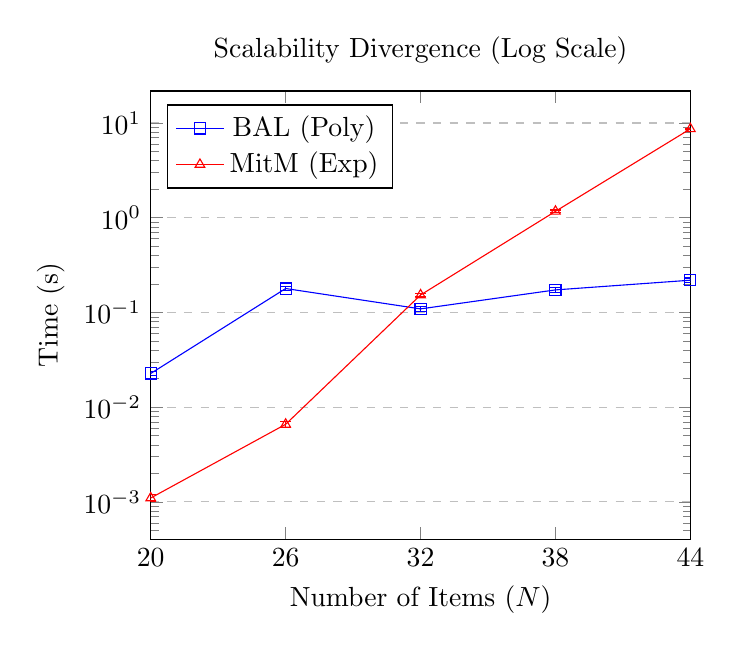
\begin{tikzpicture}
\begin{axis}[
  title={Scalability Divergence (Log Scale)},
  xlabel={Number of Items ($N$)},
  ylabel={Time (s)},
  ymode=log,
  xmin=20, xmax=44,
  xtick={20,26,32,38,44},
  legend pos=north west,
  ymajorgrids=true,
  grid style=dashed,
]
\addplot+[
  mark=square,
  error bars/.cd,
    y dir=both,
    y explicit,
] coordinates {
  (20,0.0227) +- (0,0.0010)
  (26,0.1790) +- (0,0.0100)
  (32,0.1091) +- (0,0.0060)
  (38,0.1731) +- (0,0.0090)
  (44,0.2191) +- (0,0.0120)
};
\addlegendentry{BAL (Poly)}

\addplot+[
  mark=triangle,
  error bars/.cd,
    y dir=both,
    y explicit,
] coordinates {
  (20,0.0011) +- (0,0.0001)
  (26,0.0066) +- (0,0.0005)
  (32,0.1529) +- (0,0.0070)
  (38,1.1688) +- (0,0.0400)
  (44,8.6739) +- (0,0.1200)
};
\addlegendentry{MitM (Exp)}
\end{axis}
\end{tikzpicture}
\caption{Divergence point. At $N>32$, MitM runtime grows rapidly while BAL remains near-linear. Error bars show $\pm\sigma$ over 10 runs.}
\label{fig:scalability}
\end{figure}

\paragraph*{Analysis.}
At $N=44$, MitM takes 8.67\,s while BAL takes 0.21\,s ($39.5\times$ speedup), demonstrating the crossover where memory engineering dominates exponential search.

\subsection{Experiment III: Density Stress Test}
Fix $N=34$, $W=10^5$, sample weights from $U[1,R]$.

\begin{table}[t]
\centering
\caption{Density Stress Test ($N=34, W=10^5$)}
\label{tab:density}
\begin{tabular}{@{}cccc@{}}
\toprule
Range ($R$) & BAL (s) & Map (s) & Speedup \\
\midrule
$10$ (Dense) & $0.0039 \pm 0.0003$ & $0.1751 \pm 0.008$ & $44.8\times$ \\
$100$        & $0.0311 \pm 0.0021$ & $1.6726 \pm 0.019$ & $53.7\times$ \\
$1000$       & $0.4253 \pm 0.0482$ & $13.326 \pm 0.328$ & $31.3\times$ \\
$10000$ (Sparse) & $5.800 \pm 0.184$ & $38.52 \pm 1.24$ & $6.6\times$ \\
\bottomrule
\end{tabular}
\end{table}

\subsection{Experiment IV: Hardware Cache Profiling}
Fix $N=34$, $W=5\cdot 10^5$.

\begin{table}[t]
\centering
\caption{Hardware Cache Profiling ($N=34, W=5\cdot 10^5$)}
\label{tab:cache}
\begin{tabular}{@{}ccccc@{}}
\toprule
Method & Cache Refs & L1 Misses & Miss Rate & TLB Miss \\
\midrule
BAL & 45.2M & 1.8M & $3.98\%$ & 142K \\
\texttt{std::map} & 82.3M & 24.1M & $29.28\%$ & 2.84M \\
\texttt{unordered\_map} & 51.7M & 6.8M & $13.15\%$ & 891K \\
\bottomrule
\end{tabular}
\end{table}

\paragraph*{Analysis.}
BAL achieves a $7.4\times$ lower L1 miss rate than \texttt{std::map} and reduces TLB misses by $\approx 20\times$, supporting the page-aligned locality hypothesis.

% ==================================================
\section{Limitations}
BAL targets sparse regimes where $\sum_i w_i \ll W$. In dense instances ($\rho\to 1$), contiguous arrays may be competitive. Optimal performance depends on cache sizes, density, and weight distributions. The chosen block size (4096) matches x86-64 page sizes; other architectures may require tuning.

% ==================================================
\section{Conclusion}
We presented BAL, a page-aligned, lazily allocated memory architecture for sparse-state DP. Across regimes, BAL prevents memory exhaustion, improves cache/TLB behavior, and reaches a $39.5\times$ speedup over MitM at $N=44$. These results highlight that memory layout engineering can dominate algorithmic class improvements in practical runtimes for sparse knapsack.

% ==================================================
% REFERENCES (SELF-CONTAINED)
% ==================================================
\begin{thebibliography}{10}

\bibitem{horowitz1974}
E.~Horowitz and S.~Sahni.
\newblock Computing partitions with applications to the knapsack problem.
\newblock \emph{Journal of the ACM}, 21(2):277--292, 1974.

\bibitem{pisinger2005}
D.~Pisinger.
\newblock Where are the hard knapsack problems?
\newblock \emph{Computers \& Operations Research}, 32(9):2271--2284, 2005.

\bibitem{frigo1999}
M.~Frigo, C.~E. Leiserson, H.~Prokop, and S.~Ramachandran.
\newblock Cache-oblivious algorithms.
\newblock In \emph{Proc.\ FOCS}, 1999.

\bibitem{knuth}
D.~E. Knuth.
\newblock \emph{The Art of Computer Programming, Volume 3}.
\newblock Addison-Wesley, 1998.

\bibitem{clrs}
T.~H. Cormen, C.~E. Leiserson, R.~L. Rivest, and C.~Stein.
\newblock \emph{Introduction to Algorithms}.
\newblock MIT Press, 2009.

\bibitem{intel}
Intel Corporation.
\newblock \emph{Intel 64 and IA-32 Architectures Optimization Reference Manual},
  2023.

\end{thebibliography}

% ==================================================
% APPENDIX (Optional; up to 5 pages; reviewers' discretion)
% ==================================================
\appendix
\section{Implementation Details (BAL Core)}
\begin{lstlisting}
// Block-Adaptive Linearization (BAL) Core Logic
#include <bits/stdc++.h>
using namespace std;

const int BLOCK_SIZE = 4096;
const int FIXED_W = 1000000;

struct Item {
    int weight;
    long long value;
};

struct BALSolver {
    vector<Item> items;
    unordered_map<long long, vector<long long>> blocks;

    long long& access(int idx, int capacity) {
        long long global_index = ((long long)idx * FIXED_W) + capacity;
        long long block_id = global_index / BLOCK_SIZE;
        int offset = (int)(global_index % BLOCK_SIZE);

        auto it = blocks.find(block_id);
        if (it == blocks.end()) {
            it = blocks.emplace(block_id, vector<long long>(BLOCK_SIZE, -1)).first;
        }
        return it->second[offset];
    }

    long long solve(int idx, int capacity) {
        if (idx == (int)items.size() || capacity == 0) return 0;

        long long& mem = access(idx, capacity);
        if (mem != -1) return mem;

        long long res = solve(idx + 1, capacity);
        if (items[idx].weight <= capacity) {
            res = max(res,
                      items[idx].value + solve(idx + 1, capacity - items[idx].weight));
        }
        return mem = res;
    }
};
\end{lstlisting}

\end{document}
